\section{Ansys Cases and Interface Verification}
\label{chapter:09}

% block-id: 09.ansys.p1
\hypertarget{09.ansys.p1}{}
The historical two-dimensional seven-strand port test uses 704 elements, two voltage basis solutions, and a third actual ±20 A field solution. Common terminal voltage, complex strand currents, and independent power establish field–circuit consistency on that mesh; current results appear in Fig.~\ref{fig:ansys_seven_current}. Validation concerns one mesh. Subsequent fixed-mesh and precision attempts have not completed the required three-level checks, and the native three-dimensional J-expression probe has not produced an acceptable physical solution.

% block-id: 09.ansys.p2
\hypertarget{09.ansys.p2}{}
Fig.~\ref{fig:ansys_limits} summarizes the verified Ansys Student v252 limits: up to 2000 triangles in two dimensions, 64000 volume elements and 8000 surface elements in three dimensions, and at most four processor cores. Interface capability, licensed model size and numerical accuracy separately constrain executable validation. Actual terminations, curved STL geometry and large bundles with sufficient copper area require licensing and mesh capacity appropriate to the target geometry, followed by sensitivity and power-balance checks.

% block-id: 09.figure.ansys_seven_current
\hypertarget{09.figure.ansys_seven_current}{}
\begin{figure}[!htbp]
\centering
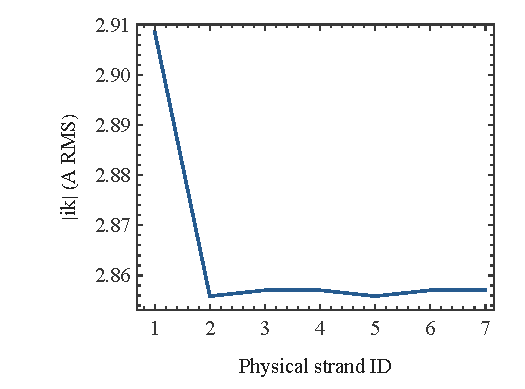
\includegraphics[width=\linewidth,height=.72\textheight,keepaspectratio]{../../assets/en/ansys_seven_current.pdf}
\caption{Ansys seven-strand two-dimensional complex currents. The valid 704-cell port short test provides strand magnitudes and phases. Currents use port records from the actual ±20 A field solution. Magnitudes and phases correspond to the same seven strand identities.}
\label{fig:ansys_seven_current}
\end{figure}

% block-id: 09.figure.ansys_limits
\hypertarget{09.figure.ansys_limits}{}
\begin{figure}[!htbp]
\centering
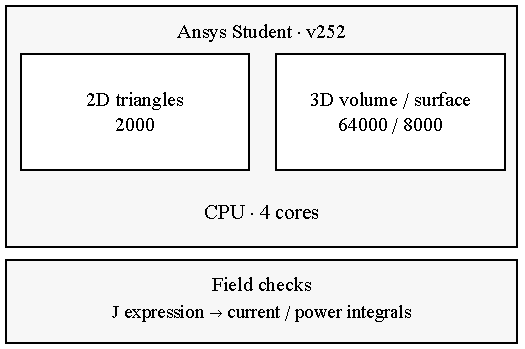
\includegraphics[width=\linewidth,height=.72\textheight,keepaspectratio]{../../assets/en/ansys_limits.pdf}
\caption{Ansys Student capacity and interface diagnostics. License capacity and field-check entry points for Ansys Student v252: 2000 triangles in two dimensions, 64000 volume and 8000 surface elements in three dimensions, and up to four compute cores. Capacity information is retained from rc.1 records; figure sources were checked on 2026-10-15.}
\label{fig:ansys_limits}
\end{figure}

% block-id: 09.ansys.rc2
\hypertarget{09.ansys.rc2}{}
The rc.2 records additionally complete two-dimensional Maxwell construction, solution, and project readback through PyAEDT-MCP, with task cancellation and linked restart records. A seven-strand straight-bundle comparison with Wolfram aligns cross-section, material, frequency, return, and total-current constraints. Relative complex-current L2 and bundle Rac differences are 0.0106814\% and 0.00132823\%, respectively. The implementations use independent meshes, Maxwell performs one adaptive pass, and spatial and boundary convergence remain to be checked. This success establishes the corresponding two-dimensional port workflow; three-dimensional interfaces and transposed structures with sufficient copper require their own field solutions and acceptance. \cite{PYAEDTMCP,PYAEDT}
